\documentclass[12pt]{article}
\setlength{\oddsidemargin}{0.50in}
\setlength{\textwidth}{5.5in}
\setlength{\topmargin}{0in}
\setlength{\textheight}{8.0in}
\usepackage{booktabs}



\newtheorem{theorem}{Theorem}
\usepackage{graphicx}
\newtheorem{lemma}{Lemma}
\newtheorem{observation}{Observation}
\newtheorem{definition}{Definition}
\newtheorem{example}{Example}
\usepackage{hyperref}
\hypersetup{
    colorlinks=true,
    linkcolor=blue,
    filecolor=magenta,      
    urlcolor=cyan,
}



\begin{document}

\begin{titlepage}
	\begin{center}
	
	
	{\Large \bf
Growing Degree Days in Canada (Group 4) \\

\vspace*{0.4in}
}
Zaynab Musa\\ 
Frazao, Fabio Soares\\
Chenxiao Jia\\
Fatima Shaheen\\
Dianlong Zhang\\
Dayo Osunrinde\\

\vspace*{0.3in}  
\textsc{\small In partial fulfilment of the requirements of CMSC 6950(Computer Based Research Tools and Application),2016}

\end{center}
\vspace*{4.7in}
\begin{flushleft}
{\textsc Memorial University of Newfoundland,} \\
\today
\end{flushleft}
\end{titlepage}

\newpage
\begin{abstract}
Growing Degree Days (GDDs) are used to estimate the growth and development of plants and insects during the growing season. Heat units expressed in growing degree days(GDDs) are frequently used to describe the timing of biological process

The objective of this paper is to calculate the GDD for selected cities in Canada. We  also provide a visual representation of the accumulated GDD for selected cities in Canada over a given period.A visual examination of the annual cycle of minimum and maximum daily temperatures for canadian cities is explored.


 Finally, we explore how the GDD calculation depends on the base temperature for selected cities in Canada.\\



 Keywords -- {\bf Growing Degree Days(GDDs)}


\end{abstract}
\newpage
\tableofcontents
\listoffigures
\newpage
\section{ \bf Introduction}

\subsection{Growing Degree Days}
The amount of heat required to move a plant or pest to the next development stage remains constant from year to year.However, the actual amount of time(days) can vary considerably from year to year because of weather conditions. Sometimes called heat units, The Growing Degree Day, or GDD, is a heat index that can be used to predict when a crop will reach maturity. Each day’s GDD is calculated by subtracting a reference temperature, which varies with plant species, from the daily mean temperature (we ignore values less than zero).  

The summation of GDD units can be used for a variety of things: comparing one region to another, comparing one season to another, and predicting important stages in plant and pest development.


\subsubsection{Growing Degree Day Equation }
Using the Averaging method, the GDD is calculated as follows:\\
$ GDD = Average Daily Temperature - Base Temperature$\\
where $Average Daily Temperature = T_{max} - T_{min} /2 $\\

We adopt the following constraints:
\begin{enumerate}
\item If $GDD < 0$, then $GDD = 0$
\item If $T_{max} > T_{upper}$ , it is set equal to $T_{upper}$
\item If $T_{max} or  T_{min}  < 50^{\circ}F or 10^{\circ}C$, it is set equal to $10^{\circ}C$
\end{enumerate}
Using Historical Climate data, we explore the following relationships using graphs:
\begin{enumerate}
\item The accumulated GDDs for selected cities in Canada over a given period
\item The GDD dependency on the base temperature for different cities in Canada
\item The Effective GDD over the island of Newfoundland and other Canadian cities.
\end{enumerate}
\subsubsection{Annual Cycle of Air Temperature}
As the Earth revolves around the Sun, locations on the surface may under go seasonal changes in air temperature because of annual variations in the intensity of net radiation.
Historical near-surface air temperature data from many cities in canada are available as time series of daily minimum and maximum temperatures. we would also examine in this paper, the annual cycle of minimum and maximum temperatures for Canadian cities

\noindent
\section{ \bf Overview}
Section 3 of this paper shows the regression summary using the cummulative GDD as the dependent variable and the year as the independent variable in St Johns over a period of 50 years. The summary is all comprehensive as it includes the  r-square, intercept and model .
Please see Figure ~\ref{fig:GDDwithTbase} for the variation of GDD with the base temperature using a range of $0-30$ in 3 selected cities. Figure ~\ref{fig:cumGDD} shows the Cummulative GDD with time for 3 cities in Canada. Figure ~\ref{fig:Minmax} shows the anuual minimum and maximum temperature in canadian cities over a period of time,Figure ~\ref{fig:linreg} shows the linear regression for the GDD in St Johns over a period of 50 years.Figure ~\ref{fig:GDD4} shows the GDD for selected canadian cities  and Figure ~\ref{fig:EffGDD} is a map that shows the effective GDD over both all of Canada and only for the island of Newfoundland
\section{\bf Optional Task 4: Regression Analysis Summary}
\begin{figure}[tb]
 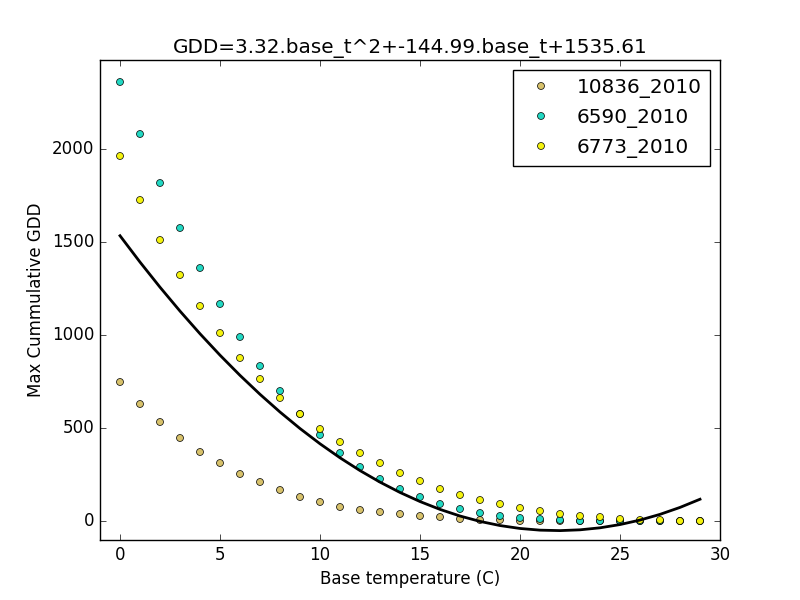
\includegraphics[width=15cm]{tbase_analysis.png}
 \caption{Variation of GDD with Tbase}
\label{fig:GDDwithTbase}
 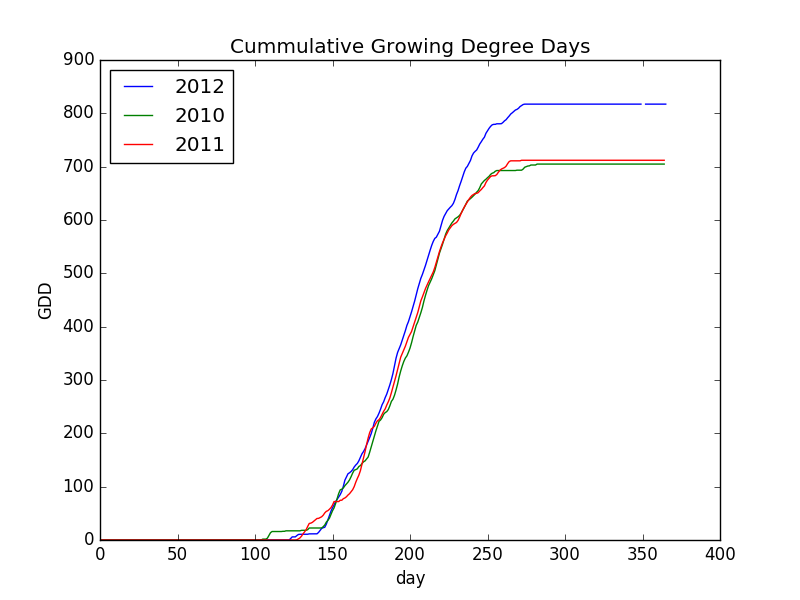
\includegraphics[width=15cm]{cummulative_GDD.png}
  \caption{Cummulative GDD }
\label{fig:cumGDD}


\end{figure}

\begin{figure}[p!]
 
 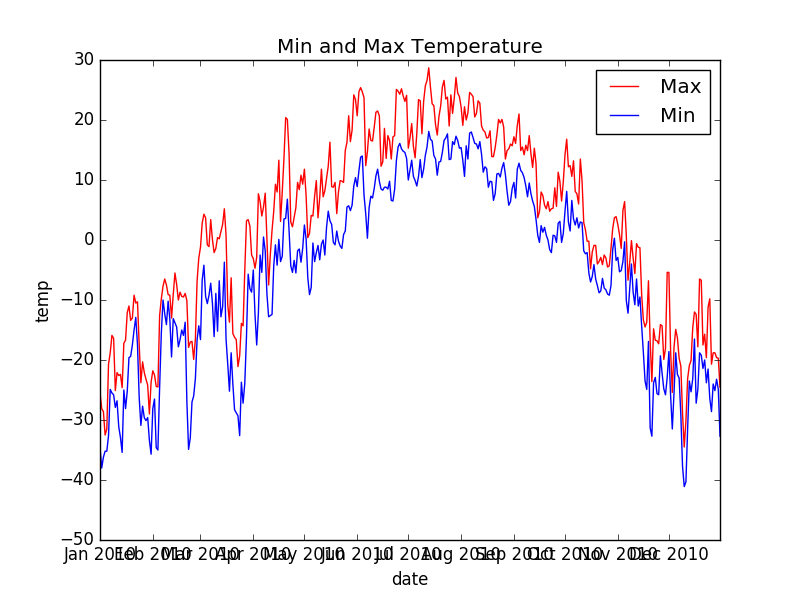
\includegraphics[width=17cm]{min_max_temperature.png}
  \caption{Annual Minimum and Maximum Temperature}
\label{fig:Minmax}
 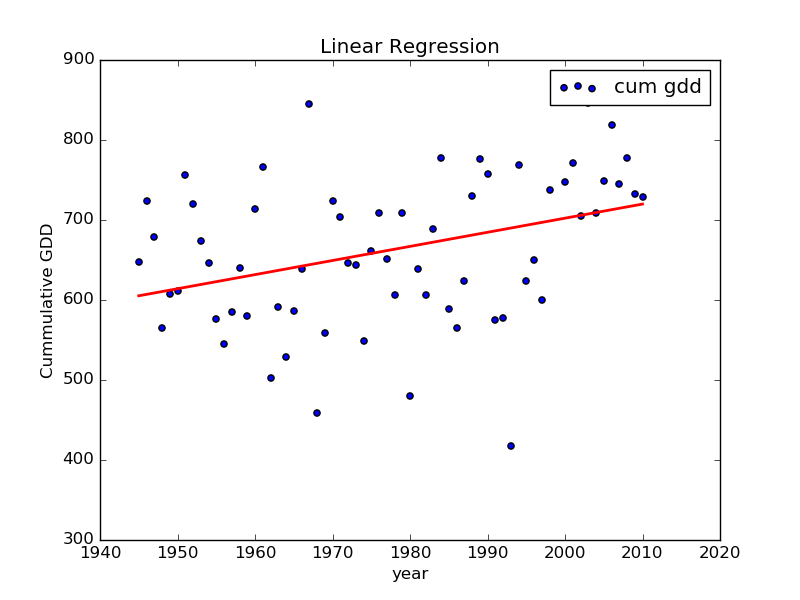
\includegraphics[width=17cm]{linear_model_plot.png}
  \caption{Linear Regression showing the best fit}
\label{fig:linreg}


\end{figure}
\begin{figure}[h!]
 
 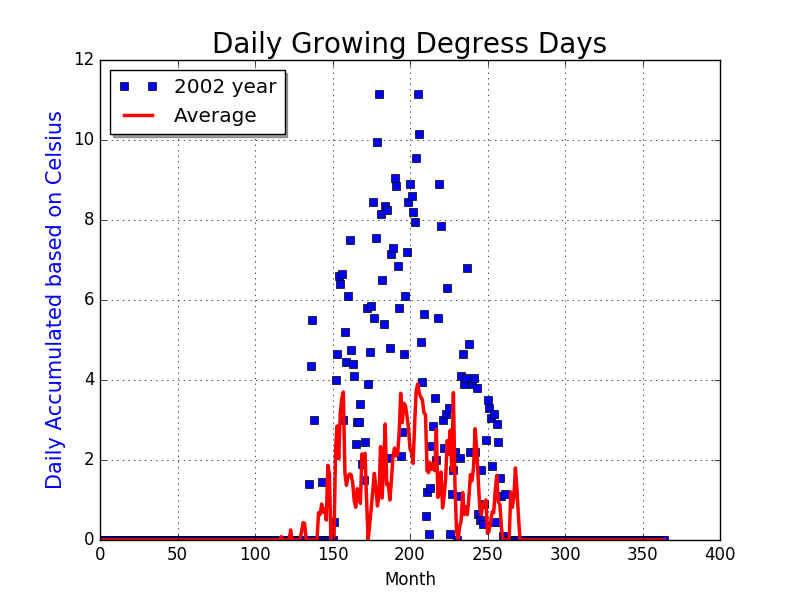
\includegraphics[width=17cm]{option1.png}
  \caption{GDD for selected Canadian Cities}
\label{fig:GDD4}
 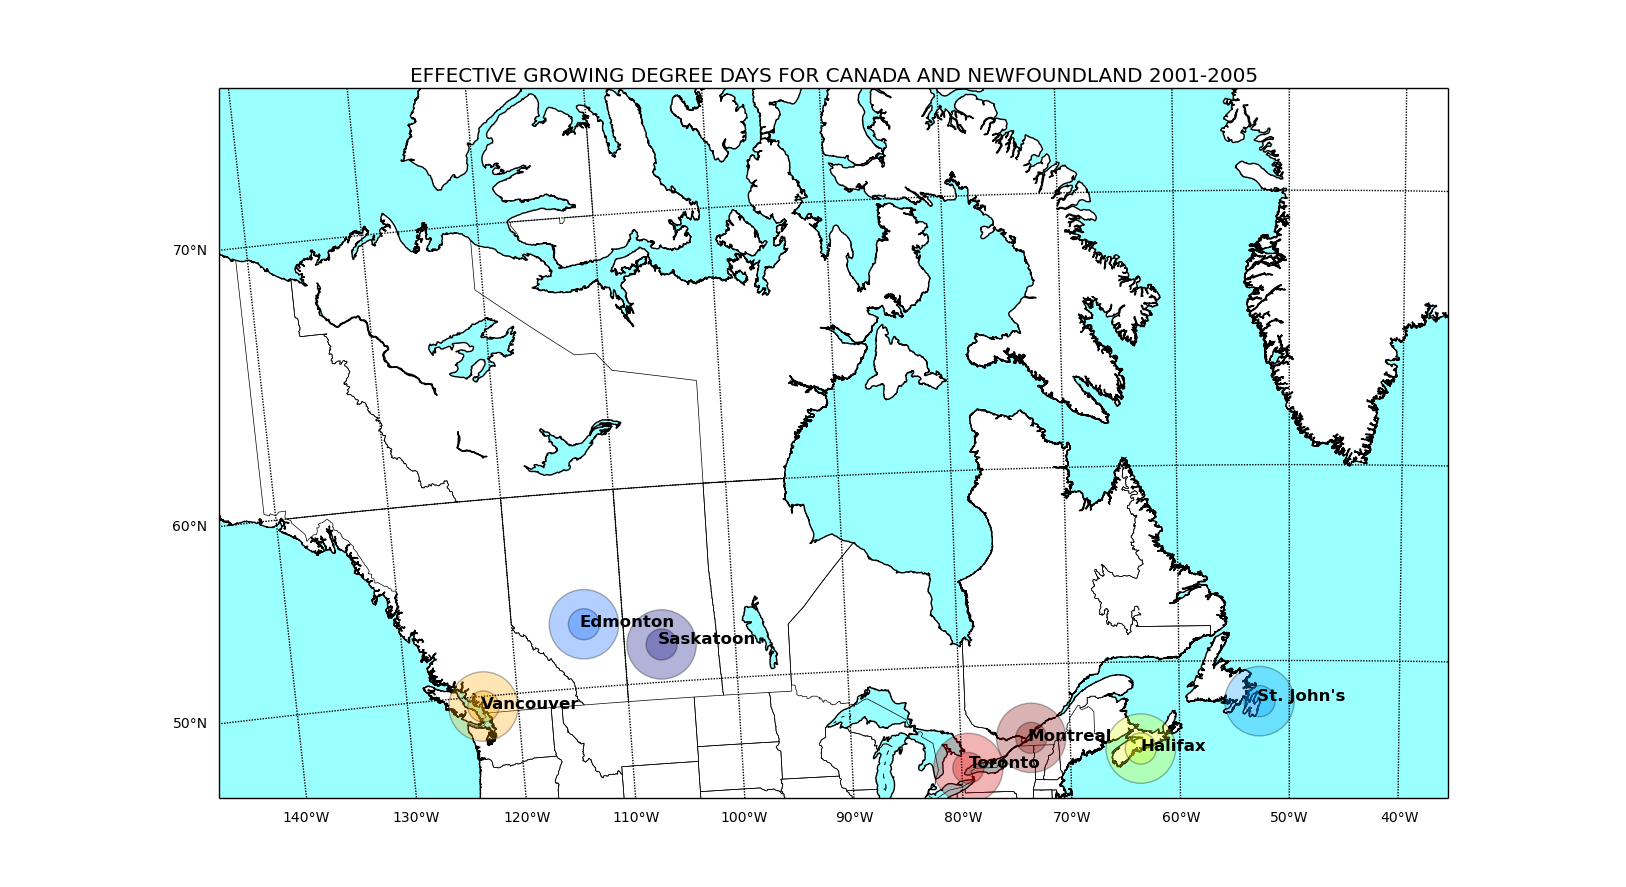
\includegraphics[width=18cm]{EffectiveGdd_1.png}
  \caption{Effective Growing Degree Days over Canada}
\label{fig:EffGDD}

\end{figure}

\begin{center}
\begin{tabular}{lclc}
\toprule
\textbf{Dep. Variable:}    &       gdd        & \textbf{  R-squared:         } &     0.124   \\
\textbf{Model:}            &       OLS        & \textbf{  Adj. R-squared:    } &     0.111   \\
\textbf{Method:}           &  Least Squares   & \textbf{  F-statistic:       } &     9.094   \\
\textbf{Date:}             & Fri, 17 Jun 2016 & \textbf{  Prob (F-statistic):} &  0.00368    \\
\textbf{Time:}             &     13:25:05     & \textbf{  Log-Likelihood:    } &   -390.01   \\
\textbf{No. Observations:} &          66      & \textbf{  AIC:               } &     784.0   \\
\textbf{Df Residuals:}     &          64      & \textbf{  BIC:               } &     788.4   \\
\textbf{Df Model:}         &           1      & \textbf{                     } &             \\
\bottomrule
\end{tabular}
\begin{tabular}{lccccc}
                   & \textbf{coef} & \textbf{std err} & \textbf{t} & \textbf{P$>$$|$t$|$} & \textbf{[95.0\% Conf. Int.]}  \\
\midrule
\textbf{Intercept} &   -2825.5110  &     1156.733     &    -2.443  &         0.017        &     -5136.351  -514.671       \\
\textbf{year}      &       1.7639  &        0.585     &     3.016  &         0.004        &         0.595     2.932       \\
\bottomrule
\end{tabular}
\begin{tabular}{lclc}
\textbf{Omnibus:}       &  2.338 & \textbf{  Durbin-Watson:     } &    1.727  \\
\textbf{Prob(Omnibus):} &  0.311 & \textbf{  Jarque-Bera (JB):  } &    1.626  \\
\textbf{Skew:}          & -0.355 & \textbf{  Prob(JB):          } &    0.443  \\
\textbf{Kurtosis:}      &  3.297 & \textbf{  Cond. No.          } & 2.05e+05  \\
\bottomrule
\end{tabular}
%\caption{OLS Regression Results}
\end{center}





\bibliographystyle{plain}

\begin{thebibliography}{99}

\bibitem{ERE 87}
McMaster GS, Wilhelm WW (1997){\em Growing degree-days: one equation, two interpretations. Agric For Meteorol} 87:291–300




\end{thebibliography}















\end{document}
